\section{Database programming}\label{sec:prog}
This section deals with populating the database, updating and deleting existing 
entries, and finally some SQL programming. Section~\ref{sec:manipulate} deals 
with the CRUD operations and is based on the file \verb|DataManipulation.sql| 
which can be seen in Appendix~\ref{app:data}. The SQL programming is covered in 
Section~\ref{sec:sql:programming} and is based on the file 
\verb|Programming.sql|, which can be seen in Appendix~\ref{app:prog}.

\subsection{SQL Data Manipulation} \label{sec:manipulate}
When inserting into the empty schema, it is necessary to insert cities as the 
first thing. Next is stations, followed by tracks, routes, trains, employees, 
etc. This is because of the relations and their total participation in each 
other. For example, a track cannot exist without having a station in each 
end.
Also, when inserting data into a relation, the values of the insert statement 
of course has to correspond with the relation design on our ER diagram.

An example of inserting cities, can  be seen in Figure~\ref{fig:ins:city}.



\begin{figure}[ht!]
    \centering
%    \lstset{numbers=none}
%    \begin{lstlisting}
%#Single insert statement
%INSERT City VALUES(4000, "Roskilde");
%#Multiple insert statements
%INSERT City VALUES
%(4320, "Lejre"), 
%(4330, "Hvalsø");
%    \end{lstlisting}
    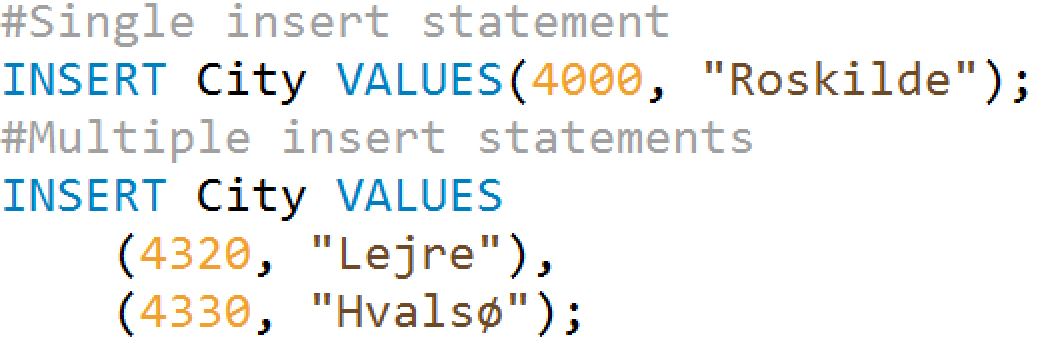
\includegraphics[scale=.5]{img/INSERT_Statements}
    \caption{SQL INSERT statements for \emph{City}.}
    \label{fig:ins:city}
\end{figure}

Once our database contains cities it is possible to insert stations located in 
these cities, which can be done as shown in Figure~\ref{fig:ins:station}.

\begin{figure}[ht!]
    \centering
    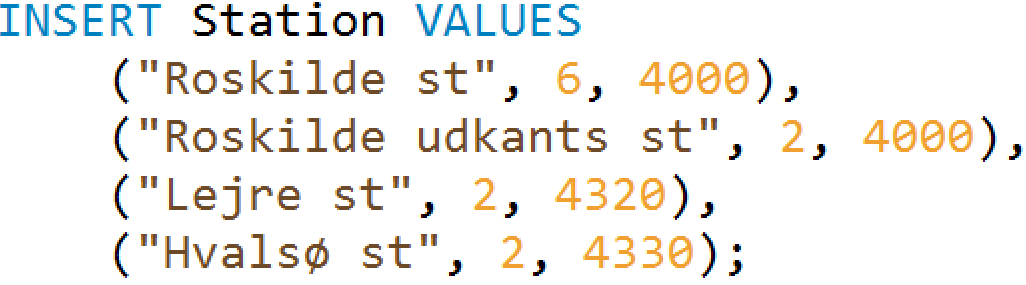
\includegraphics[scale=.5]{img/INSERT_Statement_Station}
    \caption{SQL INSERT statements for \emph{Station}.}
    \label{fig:ins:station}
\end{figure}

We can then connect the stations via tracks, effectively giving us a railway 
system, see Figure~\ref{fig:ins:track}.

\begin{figure}[ht!]
    \centering
    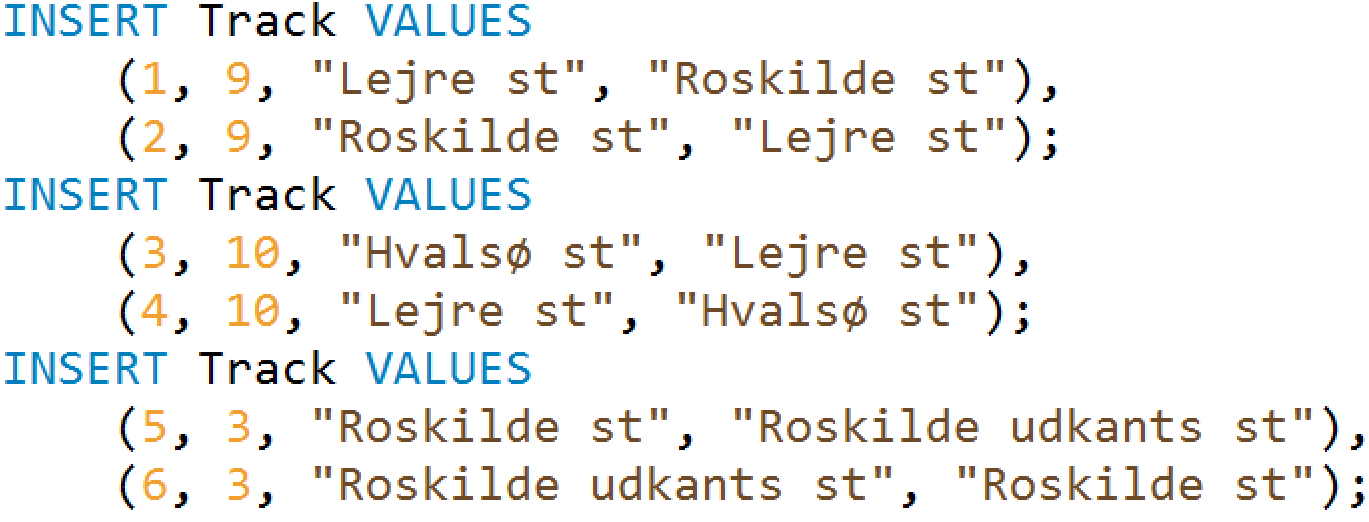
\includegraphics[scale=.5]{img/INSERT_Statements_Track}
    \caption{SQL INSERT statements for \emph{Track}.}
    \label{fig:ins:track}
\end{figure}

With the network of tracks connecting stations, we can now create routes that 
are composed of tracks. This is done in Figure~\ref{fig:ins:route}.

\begin{figure}[ht!]
    \centering
    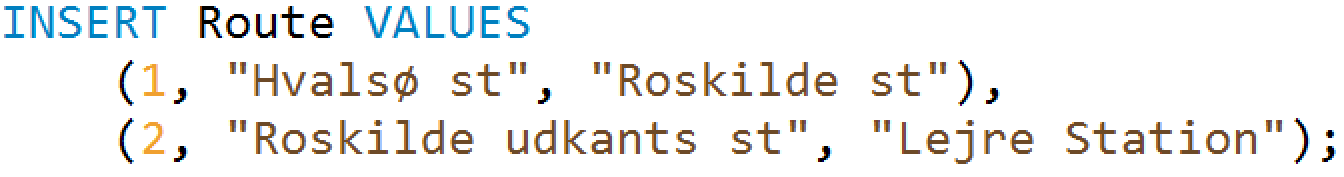
\includegraphics[scale=.5]{img/INSERT_Statements_Route}
    \caption{SQL INSERT statements for \emph{Route}}
    \label{fig:ins:route}
\end{figure}

However the routes alone, only store a start and a stop station, so clearly we 
are not done with the routes, as we still have to know which tracks each route 
is composed of. This is where the \emph{RouteTrack} relation comes in. The 
\emph{RouteTrack} table is populated in Figure~\ref{fig:ins:routetrack}.

\begin{figure}[ht!]
    \centering
    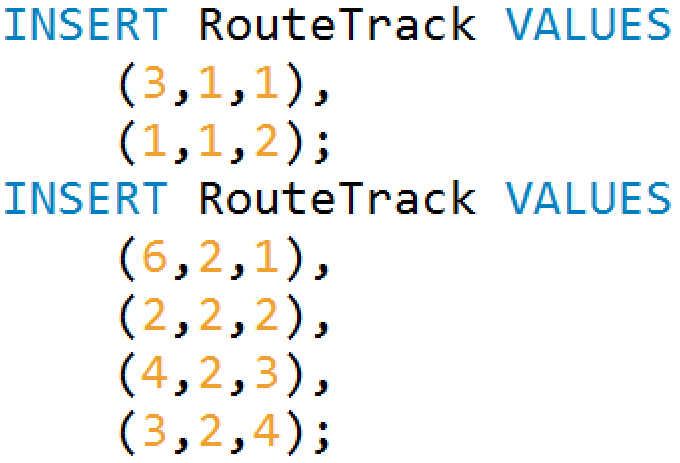
\includegraphics[scale=.5]{img/INSERT_Statements_RouteTrack}
    \caption{SQL INSERT statements for \emph{RouteTrack}.}
    \label{fig:ins:routetrack}
\end{figure}

We are now interested in having trains that drive on the tracks, following the 
routes. A train is inserted in Figure~\ref{fig:ins:train}

\begin{figure}[ht!]
    \centering
    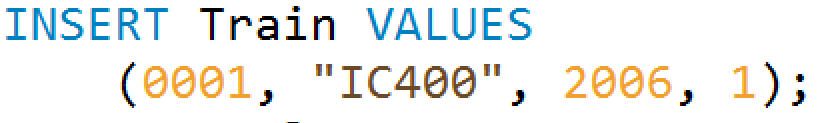
\includegraphics[scale=.5]{img/INSERT_Statements_Train}
    \caption{SQL INSERT statements for \emph{Train}.}
    \label{fig:ins:train}
\end{figure}

However, a train does not have to be on a route. Say, it could be at the 
workshop, but it is still an existing train.\todo{Move to design.}

There should of course be employees driving, maintaining, and controlling the 
trains, so we also populate the \emph{Employee} table.

\begin{figure}[ht!]
    \centering
    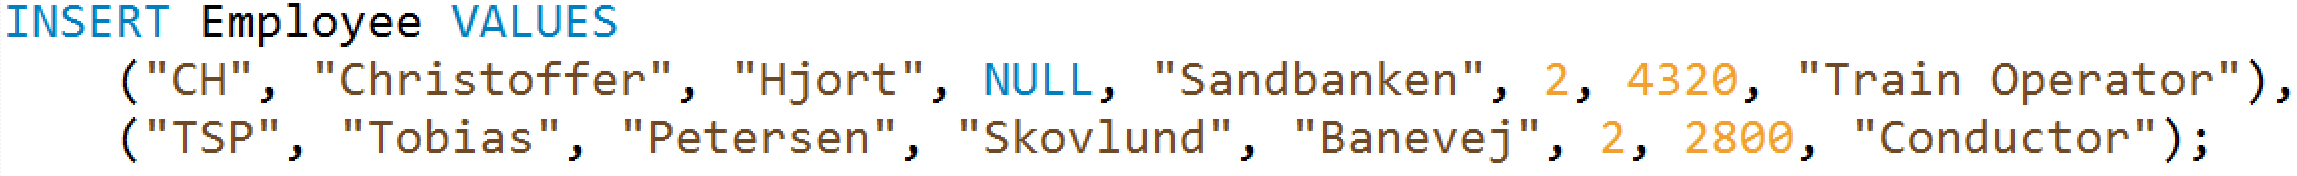
\includegraphics[scale=.5]{img/INSERT_Statements_Employee}
    \caption{SQL INSERT statements for \emph{Employee}.}
    \label{fig:ins:employee}
\end{figure}

An employee will have shifts on trains, describing when the employee is working 
on each train. A shift is stored as a tuple in the \emph{Shift} relation.

\begin{figure}[ht!]
    \centering
    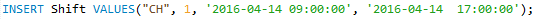
\includegraphics[scale=.5]{img/INSERT_Statements_Shift}
    \caption{SQL INSERT statements for \emph{Shift}.}
    \label{fig:ins:shift}
\end{figure}

When deleting tuples or dropping relations, the total participation of the 
relations comes into play again, just like when inserting into the schema.

In the \emph{Train Management} schema, the foreign keys with total 
participation have been set to \emph{ON DELETE CASCADE}. So, when a city is 
deleted all stations in that city are deleted as well. However, stations are 
connected through tracks and may be used as start- or end-station for a routes, 
in which case these gets deleted as well. The cascade on delete option thereby 
ripples down the database, erasing all rows that become invalid.

\begin{figure}[ht!]
    \centering
    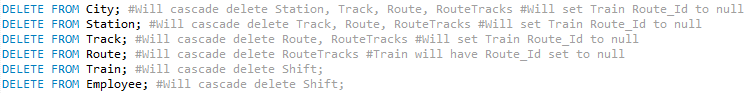
\includegraphics[scale=.5]{img/DELETE_Statements}
    \caption{SQL DELETE statements.}
    \label{fig:delete}
\end{figure}

If the foreign keys had not been set to \emph{ON DELETE CASCADE}, the relations 
would have to be deleted in correct order, starting from the bottom of 
Figure~\ref{fig:delete}.
Updates do not cascade, as the primary keys should never need to be changed. 
ID's should always stay the same, so ``should'' city zip codes and station 
names. However, foreign keys might change as for instance is a train is moved 
to drive on another route. The trains reference to a route is changed. But in 
this case a cascading action is not needed as the route does not have 
references to the trains driving on them. And since our database does not 
contain any tables with mutual references (recall that such relations were made 
into separate tables), there will never be a need for cascading after updating 
a non primary key attribute. Common update operations can be seen in 
Figure~\ref{fig:update}.

\begin{figure}[ht!]
    \centering
    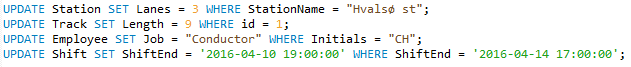
\includegraphics[scale=.5]{img/UPDATE_Statements}
    \caption{SQL UPDATE statements.}
    \label{fig:update}
\end{figure}

Some of the information that should be retrieved according to the design, 
turned out to be inconvenient to model directly, as for instance the length 
of a route. The entity \emph{Route} could have had an attribute with the length 
of the entire route, but this would be compromising the normalisations as the 
value should be calculated as the sum of lengths of all the tracks on the 
route. We therefore created the a view, that shows the length of all the 
tracks. The view, together with its implementation, can be seen in 
Figure~\ref{fig:length}.

\begin{figure}[h]
    \centering
    \begin{subfigure}[b]{0.45 \textwidth}
        \centering
        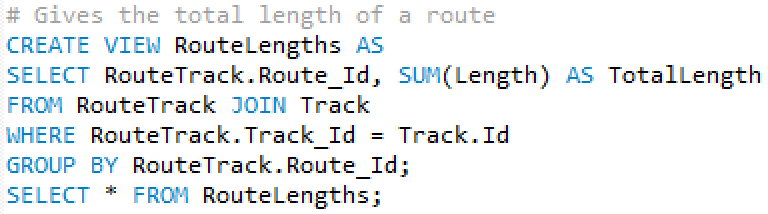
\includegraphics[width=\textwidth]{img/RouteLengths}
        \caption{Implementation of the view.}
    \end{subfigure}
    \begin{subfigure}[b]{0.45 \textwidth}
        \centering
        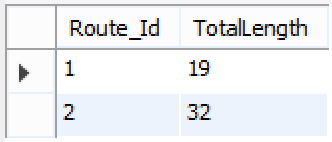
\includegraphics{img/RouteLengthsView}
        \caption{Selecting everything from the view.}
    \end{subfigure}
    \caption{View for finding the lengths of all routes.}
    \label{fig:length}
\end{figure}

Having implemented the first view we proceeded to implement views to get all 
the stations on a certain route. However, this turned out to be a fencepost 
problem, since we get the stations on the route, through the \emph{Track} 
entity. By selecting either the \emph{FromStation} or the \emph{ToStation} from 
all the tracks on the route, we would be missing either the first or the last 
station. We instead chose to select both and thus have a table of tracks 
(defined by pairs of stations), rather than stations. An example of this can be 
seen in Figure~\ref{fig:route}. Here the result is ordered by the attribute 
\emph{Number} which assures the tracks are listed in proper order (assuming of 
course that these numbers have been set properly). These two views can be used 
as if they were tables in further SQL statements. This can for instance be used 
to naturally join the view \emph{RouteLengths} with the table \emph{Routes}, 
thus adding a column with the routes length to the \emph{Routes} table. The 
column is of course only added in the result of the query and not actually 
added to the table, as that would be undesirable. This means that if a track on 
the a route changes length, then so does the length of the route, as long as 
the view is recomputed.

\begin{figure}[h]
    \centering
    \begin{subfigure}[b]{0.45 \textwidth}
        \centering
        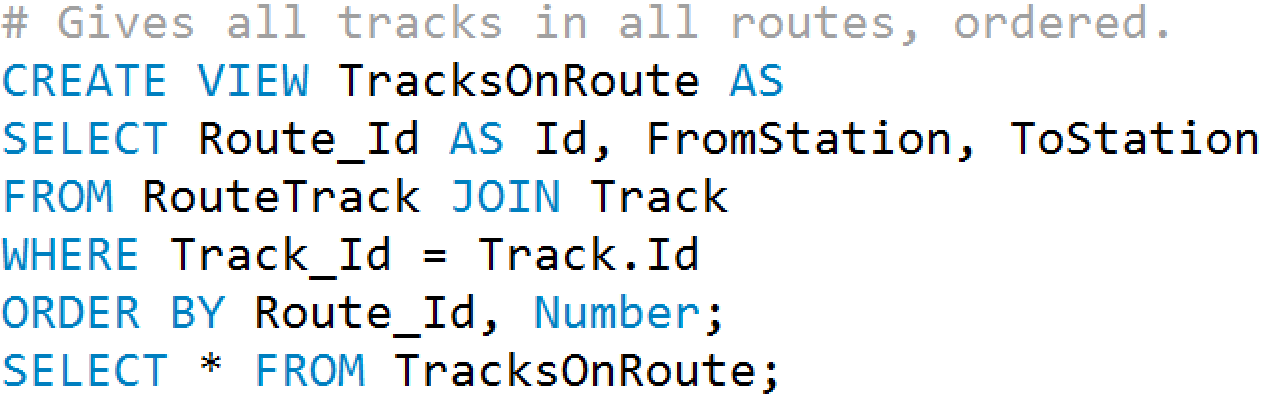
\includegraphics[width=\textwidth]{img/TracksOnRoute}
        \caption{Implementation of the view.}
    \end{subfigure}
    \begin{subfigure}[b]{0.45 \textwidth}
        \centering
        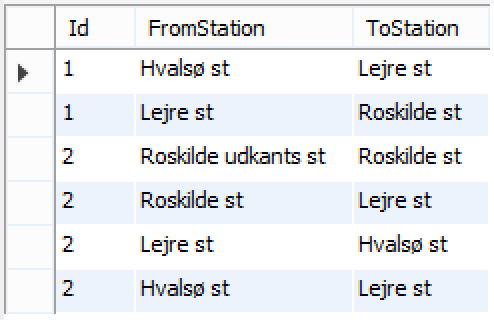
\includegraphics{img/RouteView}
        \caption{Selecting everything from the view.}
    \end{subfigure}
    \caption{View of all tracks on all routes.}
    \label{fig:route}
\end{figure}

\subsection{SQL Programming} \label{sec:sql:programming}
To control the data integrity and make insertion easier and less trivial or 
calculating attributes, a couple of functions, triggers, procedures, 
transactions and events have been programmed and implemented.

Each station has a specific capacity, that is amount of lanes. And, to make 
sure that no more tracks are connected to a station than there is capacity for, 
a trigger has been implemented to prevent insertion.

\begin{figure}[ht!]
    \centering
    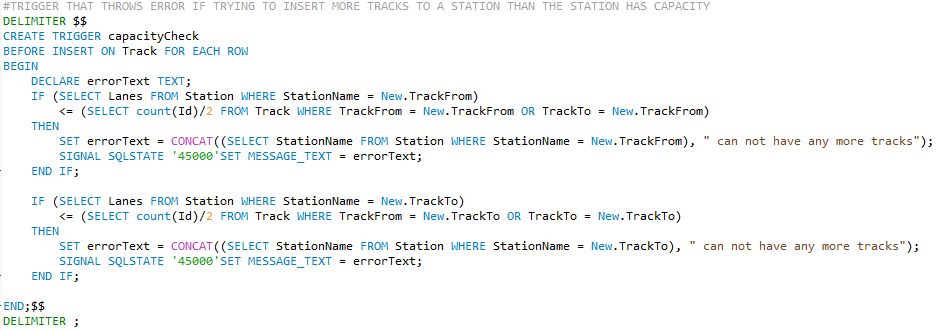
\includegraphics[scale=.75]{img/SQL_TRIGGER}
    \caption{SQL Trigger.}
    \label{fig:trigger}
\end{figure}

For example, if Station A has two lanes, which enables up to four tracks (for 
each lane there can be one ingoing and one outgoing track), and it insertion of 
a fifth track is attempted, then the trigger will throw an error 1644, and 
prevent insertion of the track. The implementation of the trigger can be seen 
in Figure~\ref{fig:trigger}

\begin{figure}[ht!]
    \centering
    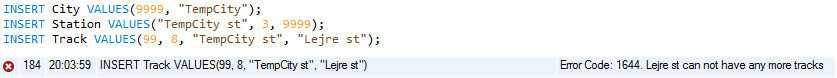
\includegraphics[width=\textwidth]{img/SQL_TRIGGER_example}
    \caption{SQL Trigger disabling insertion.}
    \label{fig:trigger2}
\end{figure}

Lejre st has 2 lanes and already has 4 tracks connected, so trying to connect a 
fifth resulted in an error from the trigger which is run \emph{BEFORE INSERT}. 
The result of this attempted insertion is illustrated in 
Figure~\ref{fig:trigger2}.

A couple of functions have also been implemented. They are primarily used to 
calculate dynamic attributes for the entities, as dynamic values should not be 
stored in a database. The first function, shown in Figure~\ref{fig:func:length} 
calculates the length of a route. This information can also be retrieved 
through the view seen in Figure~\ref{fig:length}, but has here been implemented 
to show the functionality of function. They do also differ in hat the function 
finds the length of a single route (id supplied as a parameter), whereas the 
view gives the length of all routes (from which the length of a single route 
can of course be obtained).

\begin{figure}[ht!]
    \centering
    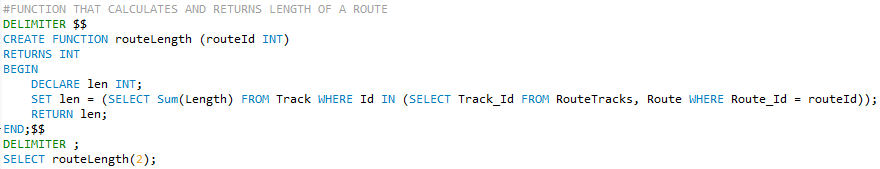
\includegraphics[scale=.75]{img/SQL_FUNCTION_Length}
    \caption{SQL Function for Track Length}
    \label{fig:func:length}
\end{figure}

Our design also required us to have the age of a train, but as this is clearly 
not a static value, it needs to be computed every time it is needed, in order 
for the value to always to accurate. This is achieved through the function 
shown in Figure~\ref{fig:age}, which simply subtracts the production year of 
the train from the current year. 

\begin{figure}[ht!]
    \centering
    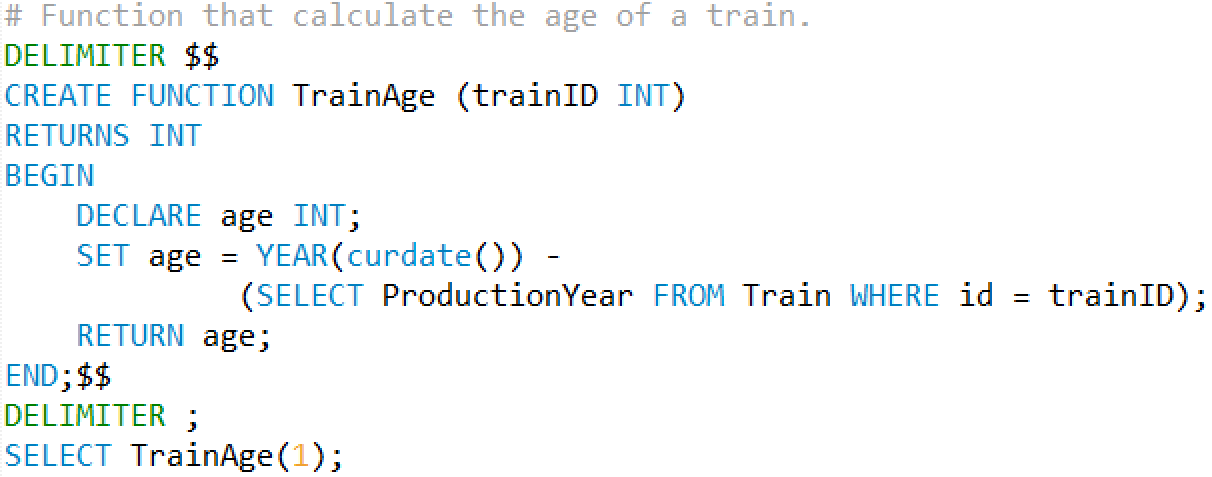
\includegraphics[scale=.75]{img/SQL_FUNCTION_Age}
    \caption{SQL Function for Train Age}
    \label{fig:age}
\end{figure}

Besides functions and triggers, we also implemented procedures. Some of the 
procedures simply reads from the tables, while other procedures also perform 
data manipulations. The procedure in Figure~\ref{fig:neighbors} finds all the 
stations neighbouring the given station. Where neighbouring is defined as; 
directly connected through a single track.

\begin{figure}[ht!]
    \centering
    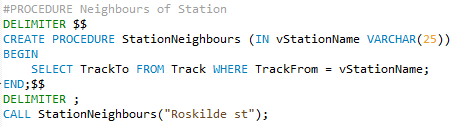
\includegraphics[scale=.75]{img/SQL_PROCEDURE_Neighbours}
    \caption{SQL Procedure for finding Station neighbours}
    \label{fig:neighbors}
\end{figure}

\begin{figure}[ht!]
    \centering
    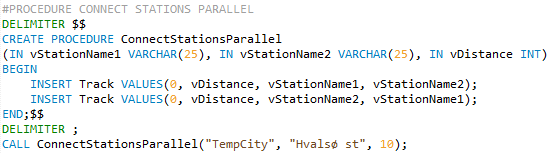
\includegraphics[scale=.75]{img/SQL_PROCEDURE_ConnectParallel}
    \caption{SQL Procedure for connecting stations parallel both ways}
    \label{fig:connectstation}
\end{figure}

The procedure inputs 0 to the ID's of the tracks, because our ID's 
automatically increments from the newest ID.

In this last procedure, a transaction has been included. This is to make sure, 
that the city and station do not get inserted unless it is possible to connect 
it to the targeted station.

\begin{figure}[ht!]
    \centering
    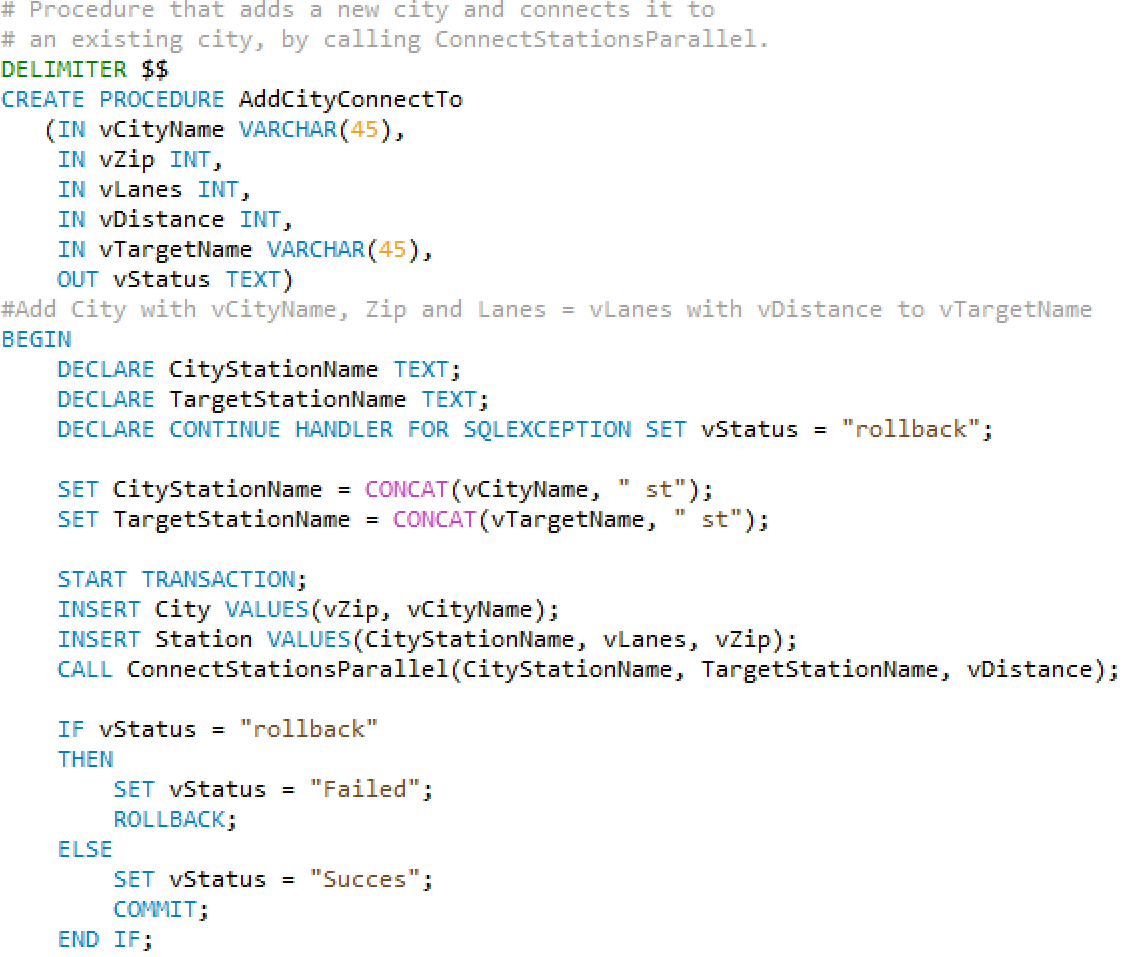
\includegraphics[scale=.75]{img/SQL_PROCEDURE_AddCityConnect}
    \caption{SQL Procedure for connecting new city to target city.}
    \label{fig:connectcity}
\end{figure}

The procedure adds a new city to the database, creates the main station for the 
city, and connects it to the specified existing target city, with a specified 
distance, by adding tracks between them.

\begin{figure}[ht!]
    \centering
    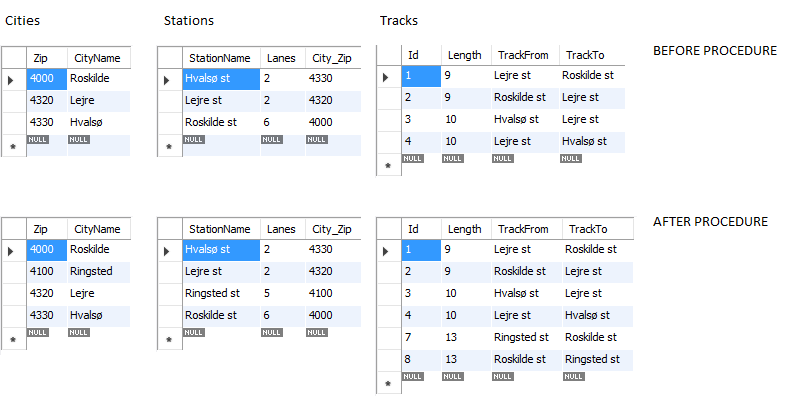
\includegraphics[scale=.75]{img/SQL_PROCEDURE_AddCityConnect_example}
    \caption{Effect of \emph{AddCityConnectTo} on database instance.}
\end{figure}
\label{fig:effect}

From the example above, the method above clear makes it quicker to insert and connect to an existing station, while still being able to specify the length of the tracks.

The only event, is really not a required functionality, as our \emph{Train 
Management} schema really has no need of events in its current state. 

\begin{figure}[ht!]
    \centering
    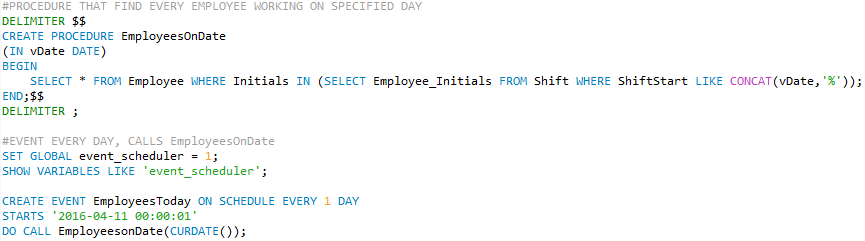
\includegraphics[scale=.75]{img/SQL_EVENT}
    \caption{SQL Event for finding todays employees}
    \label{fig:event}
\end{figure}

This event tells who is at work everyday.
The implemented event, is more for general managing, as it is nice to know for 
each day of the week what employees are at work.
